\begin{figure}[tb]
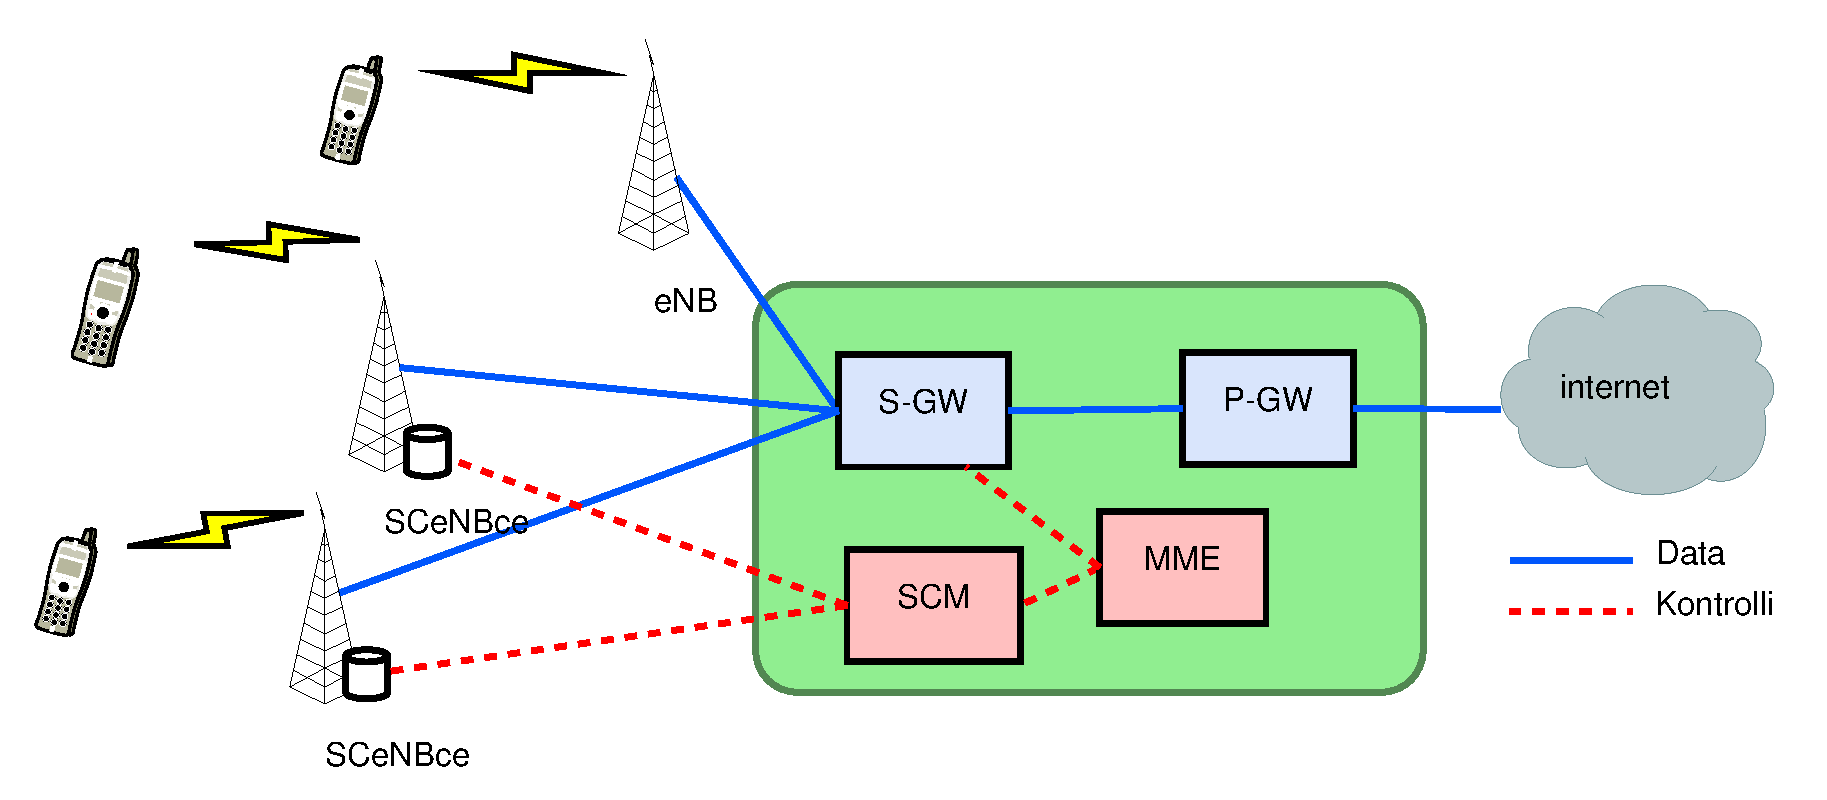
\includegraphics[width = \textwidth]{SCC.eps}
\caption{SCC arkkitehtuuri jossa SCM on integroitu osaksi EPC:tä} \label{fig:scc}
\end{figure}

\subsection{Small Cell Cloud} \label{scc}

Small Cell Cloud (SCC) on reuna-arkkitehtuuri ehdotus LTE tyyppiseen mobiiliverkkoon.
Idean premisseinä toimivat laskentaresurssien lisääminen mobiiliverkon tukiasemiin ja mobiiliverkon solujen pienenminen.
Näillä toimilla voitaisiin vastata tietoliikenteen määrän kasvuun sekä tarjota reunalaskentaa uutena palveluna.
SCC:n ratkaisuympäristönä toimii LTE verkko, jonka kehitystä ehdotettu ratkaisu pyrkii myötäilemään.
Pienemmät solut tarkoittavat että tukiasemat sijaitsevat lähempänä asiakasta, joka puolestaa implikoi asiakaslaitteille nopeampaa tiedonsiirtoväylää radiorajapinnassa \cite{lobillo15scc}.
Seuraavaksi käsitellään SCC:n toiminnallisuus aloittaen läpikäynti toimijoista. Lopuksi käsitellään tietoliikenneratkaisuja joita SCC:n yhteydessä on ehdotettu.

SCC:ssä laskentaresurssit on sijoitettu eNodeB tukiasemiin. SCC:n tapauksessa puhutaan SCeNBce:stä (Small-cell eNodeB computing-enhanced), eli laskentaresursseilla varustetusta piensolutukiasemasta \cite{lobillo15scc}.
Reunalaskentaan käytettävät resurssit ovat integroituina osaksi tukiasemaa \cite{puente15seamless}.
Ajatuksena on että tukiaseman toiminnot suoritettaisiin samalla laitteistolla kuin reunasovellukset.
Tämänkaltainen menettely mahdollistaa tukiaseman ja reuna-alustan yhteistoiminnallisuutta.
Yhteistoiminta mahdollistaa esimerkiksi radiorajapinnasta saatavien tietojen hyödyntämisen osana etälaskennan kannattavuuden päättelyä.
Lisäksi yhteisillä jaetuilla resursseilla vältyttäisiin erillisen laitteiston lisäämiseltä \cite{puente15seamless}.

SCC:n hallinnollisista toimista vastaava entiteetti on Small Cell Manager (SCM) \cite{lobillo15scc}.
SCM olisi MME:n kaltainen itsenäinen toimija, mutta vastaisi reunalaskentaan liittyvistä hallinnollisista toimista.
Tarkoituksena on että SCM on tietoinen reunasolmujen resurssien tilasta ja on kykenevä tekemään päätöksia reunasovelluksien siirtämisestä sijainnista toiseen. 
Lisäksi SCM:n tehtävänä on vastata muun muassa asiakaslaitteiden pyyntöihin laskentaresursseista osoittamalla käytettävissä oleva virtuaalikone \cite{dolezal2016performance}.
SCM voi myös sähkön säästämiseksi sulkea SCeNBce:n reunalaskentatoiminnallisuuden.
SCM:n sijoittelu mobiiliverkon sisällä on jätetty toteuttajan vastuulle, mutta ehdotettuja sijainteja ovat muun muassa MME:n yhteydessä ja täysin itsenäisenä toimijana \cite{lobillo15scc}.
SCM toteutusvaihtoehdot sisältävät sekä hajautettuja että keskitettyjä malleja.

SCC ympäristössä perustoiminnallisuus menisi siten että reunalaskentaa tahtova asiakaslaite välittäisi pyynnön SCeNBce:lle joka edelleen välittäisi pyynnön SCM:lle.
SCM toimii reuna-alustan roolissa ja valitsee SCeNBce:lle virtuaalikoneen, jolla reunlaskentaa voidaan suorittaa. \cite{dolezal2016performance}


Koska SCC:n ehdotetaan olevan tiukasti integroituna LTE mobiiliverkkoon, vaatii se olemassa olevien rajapintojen lisäksi uuden rajapinnan SCM vaatimien toiminnallisuuksien toteuttamiseksi. SCM tarvitsee rajapinnan MME:hen jonka kautta se voi esimerkiksi autentikoida asiakaslaitteita \cite{lobillo15scc}. 
Joskaan SCC:n käyttöönotto ei vaadi mobiiliverkon täysimittaista uudelleen rakentamista, edellyttää se toimiakseen ainakin olemassa olevien tukiasemien korvaamisen SCeNBce tyyppisillä tukiasemilla. Lisäksi käyttöönotto vaatii puuttuvien rajapintojen lisäämistä MME:n yhteyteen. 
Laskentaresurssien sijoittaminen tukiasemaan tekee resursseista hyvin paikallisesti hyödynnettäviä. Onkin siis tarkkaan pohdittava resurssien määrää tukiasemassa koska ne eivät ole kovin helposti muiden solujen hyödynnettävissä.
%täten voi oletta

 
%
%SCC:n arkkitehtuurin haasteena saattaa olla niiden ylläpidettävyys, jossa matkapuhelinverkko-operaattori on vastuussa reunasolmun ylläpidosta, koska se on tiukasti sidoksissa tukiasemaan\cite{lobillo15scc}.
%Tukiasemaan tiukasti sidotulla ratkaisulla on kuitenkin mahdollista hyödyntää laajemmin tukiaseman ominaisuuksia, kuten radioyhteyksiä toisiin tukiasemiin.
%SCeNBce tukiasemien hankkiminen vaatii operaattoreilta investointeja sekä lisää ylläpitotyön määrää. (Näiden vuoksi ehkä kantsis miettii, että miksi se on niin tiukasti kiinni siinä televerkossa. Muutenkin useampi operaattori samalla alueella tarkoittaa että jokaisella on myös omat reunapalvelut, joka taas meinaa kokonaiskuvassa että sama palvelu pitää duplikoida monelle operaattorille.)

\subsubsection{Kommunikointi reunapalveluun} \label{GTP}
Kuten kappaleessa \ref{kommunikaatio} käsiteltiin, tavallisesti asiakaslaitteen tietoliikenne kulkee mobiiliverkon läpi koskemattomana GTP tunnelin sisällä. 
SCC:n asiakaslaitteen ja reunalaskennan välisen tietoliikenteen reititys on esitelty julkaisussa \cite{puente15seamless}, johon tämä kappale pohjautuu.
SCC:n tapauksessa asikaslaitteen liikenne haluttaisiin ohjata kohteesta riippuen joko tukiasemassa sijaitsevalle reunasolmulle tai normaalia reittiä pitkin ulkoverkkoon.
SCC:ssä on päädytty lisäämään SCeNBce tukiasemaan tietoliikennettä monitoroiva toiminnallisuus.

Kommunikaatio asiakaslaitteen ja tukiaseman välillä suoritetaan DRB väylällä (Data Radio Bearer).
Perinteisesti tukiasema identifioi asiakaslaitteet radiorajapinnassa DRB ID:n (Data Radio Bearer ID) avulla.
Tämän jälkeen asiakaslaitteen tietoliikenne on tukiasema kapseloi asiakkaan tietoliikenteen GTP tunneliin, jonka tunnisteena toimii TEID (Tunnel Endopoint ID).
Asiakaslaitteen tietoliikenteen välitys tukiaseman sisällä vaatii siis DRB ID:n ja TEID:n sisältävän muunnostaulun käyttämistä.
Tätä samaa periaatetta voi hyödyntää reunasolmulle suuntautuvan tietoliikenteen identifiointiin.

Tukiasemaan lisättävän monitoritoiminnallisuus tarkkailee asiakaslaitteen lähettämien pakettien kohde IP-osoitetta, ja mikäli kyseessä on reunapalvelun IP-osoite, monitori ohjaa paketin reunapalvelulle.
Samalla paketista voidaan poimia asiakaslaitteen IP-osoite, joka kirjataan muunnostauluun asiakasta vastaavan TEID:n ja DRB ID:n kanssa.
Toiseen suuntaan tietoliikenne toimii siten että reunapalvelun asiakaslaitteelle lähettämästä tietoliikenteestä poimitaan kohde IP. Kohde IP:tä vastaava DRB ID poimitaan muunnostaulusta reunapalvelun paketit kapseloidaan DRB väylälle sopiviksi.
Tällaisen toiminnallisuuden toteuttamisen seurauksena kommunikaatio on asiakaslaitteen ja reunapalvelun näkökulmasta kuin mikä tahansa muukin IP-pohjainen kommunikaatio.

Asiakaslaiteen ja reunasolmun välisen kommunikaation säilymiseen, tilanteessa, jossa asiakaslaite siirtyy toiselle tukiasemalle, ei oteta kantaa. 
Tällaisen toiminnallisuuden tarve kuitenkin on, sillä SCM esittelyn yhteydessä mainittiin reunasovelluksien, eli virtuaalikoneiden, siirtelyn mahdollisuus.
%SCC pohjaisessa järjestelmässä tavallinen verkkoon menevä tietoliikenne ja reunapalvelulle menevä tietoliikenne on ehdotettu eroteltavaksi toisistaan \cite{puente15seamless}.
%Eristyksen seurauksena LTE-A arkkitehtuuriin ei tarvitse koskea muutoin kuin lisäyksien osalta. 
%Liikenne SCeNBce:llä tarjottuihin reunapalveluihin on tehtävä tarkoitusta varten olevan rajapinnan kautta.
%Asiakaslaitteelta tuleva liikenne reititetään SCeNBce:llä. 
%Pakettien reitittämiseksi SCeNBce joutuu päättelemään, onko paketin määränpää reunapalvelu vai tavallinen tietoliikenne.
%
% Koska LTE-tukiasemat eivät toimi IP tasolla, ei reunapalvelulta tuleva pakettiliikenteen sisältämä asiakaslaitteen IP-osoite riitä identifioimaan kohdelaitetta. 
%Yleisesti LTE verkossa, internetistä asiakaslaitteelle suuntautuvan liikenteen osalta pakettien ohjaamiseksi, käytetään GTP-tunnelia. GTP-tunnelilla tietoliikenne saadaan ohjattua oikealle tukiasemalle.
%Tukiaseman ja asiakaslaitteen välisen kommunkaatioväylän selvittämiseksi joudutaan tekemään TEID (Tunnel endpoint IDentifier) ja DRB-ID (Data Radio Bearer ID) muunnos.
%
%Vastaava ongelma on myös reunapalvelulta asiakaslaitteelle suuntautuvassa tietoliikenteessä.
%SCC:n yhteydessä ehdotetussa ratkaisussa reunapalvelulta tulevan liikenteen yhdistäminen asiakaslaitteen IP-osoitteeseen voidaan tehdä käyttäen TEID perustuvaa ohjaustaulua.
%TEID on asiakaskohtaisen GTP-tunnelin indetifioiva tunniste.
%TEID:stä ja asiakaslaitekohtaisesta IP-osoitteesta voidaan muodostaa SCeNBce:lle reititystaulu. 
%Reititystaulun avulla voidaan ohjata IP-osoitte muuntaa DRB liikkenneväyläksi ja ohjata tietoliikenne asiakaslaitteeseen.

